
\begin{figure}[h!]
\def\bb{\rule{2in}{0pt}\rule{0pt}{1in}}
\def\lp#1[#2]#3{\parbox{0.16\linewidth}{\labelledpic{#1}{\includegraphics[#2]{#3}}}}
\begin{tabular}{cccccc}
\includegraphics[trim={0 2cm 0 1.25cm},clip,width=0.16\linewidth]{res_bear_new/rgb.jpg} & 

\includegraphics[trim={0 2cm 0 1.25cm},clip,width=0.16\linewidth]{res_bear_new/target.jpg} & 
\includegraphics[trim={0 2cm 0 1.25cm},clip,width=0.16\linewidth]{res_bear_new/heatmap.jpg} & 
\includegraphics[trim={0 2cm 0 1.25cm},clip,width=0.16\linewidth]{res_bear_new/cleaned_skeleton_sil.jpg} &
\includegraphics[trim={0 2cm 0 1.25cm},clip,width=0.16\linewidth]{res_bear_new/3d_fit_overlay_rgb.jpg} & 
\includegraphics[trim={0 2cm 0 1.25cm},clip,width=0.16\linewidth]{res_bear_new/3d_fit_reversed.jpg} \\

\includegraphics[trim={0 0.5cm 0 0.5cm},clip,width=0.16\linewidth]{res_horse_new/rgb.jpg} & 

\includegraphics[trim={0 0.5cm 0 0.5cm},clip,width=0.16\linewidth]{res_horse_new/target.jpg} & 
\includegraphics[trim={0 0.5cm 0 0.5cm},clip,width=0.16\linewidth]{res_horse_new/heatmap.jpg} & 
\includegraphics[trim={0 0.5cm 0 0.5cm},clip,width=0.16\linewidth]{res_horse_new/cleaned_skeleton_sil.jpg} &
\includegraphics[trim={0 0.5cm 0 0.5cm},clip,width=0.16\linewidth]{res_horse_new/3d_fit_overlay_rgb.jpg} & 
\includegraphics[trim={0 0.5cm 0 0.5cm},clip,width=0.16\linewidth]{res_horse_new/3d_fit_reversed.jpg} \\

\includegraphics[trim={0 1.5cm 0 1.5cm},clip,width=0.16\linewidth]{res_rsdog158_new/rgb.jpg} & 

\includegraphics[trim={0 1.5cm 0 1.5cm},clip,width=0.16\linewidth]{res_rsdog158_new/target.jpg} & 
\includegraphics[trim={0 1.5cm 0 1.5cm},clip,width=0.16\linewidth]{res_rsdog158_new/heatmap.jpg} & 
\includegraphics[trim={0 1.5cm 0 1.5cm},clip,width=0.16\linewidth]{res_rsdog158_new/cleaned_skeleton_sil.jpg} &
\includegraphics[trim={0 1.5cm 0 1.5cm},clip,width=0.16\linewidth]{res_rsdog158_new/3d_fit_overlay_rgb.jpg} & 
\includegraphics[trim={0 1.5cm 0 1.5cm},clip,width=0.16\linewidth]{res_rsdog158_new/3d_fit_reversed.jpg} \\

\lp a[trim={0 1cm 0 1cm},clip,width=0.98\linewidth]{res_camel_new/rgb.jpg} & 
\lp b[trim={0 1cm 0 1cm},clip,width=0.98\linewidth]{res_camel_new/target.jpg} & 
\lp c[trim={0 1cm 0 1cm},clip,width=0.98\linewidth]{res_camel_new/heatmap.jpg} & 
\lp d[trim={0 1cm 0 1cm},clip,width=0.98\linewidth]{res_camel_new/cleaned_skeleton_sil.jpg} &
\lp e[trim={0 1cm 0 1cm},clip,width=0.98\linewidth]{res_camel_new/3d_fit_overlay_rgb.jpg} & 
\lp f[trim={0 1cm 0 1cm},clip,width=0.98\linewidth]{res_camel_new/3d_fit_reversed.jpg} 
\end{tabular}
\caption{Example results on various animals. From left to right: RGB input, extracted silhouette, network-predicted heatmaps, OJA-processed joints, overlay 3D fit and alternative view.}
\label{fig:example_results}
\end{figure}